\documentclass[11pt,a4paper]{article}
\usepackage[utf8]{inputenc}
\usepackage[vietnamese]{babel}
\usepackage{amsmath,amssymb}
\usepackage[version=4]{mhchem}
\usepackage{geometry}
\geometry{top=1.5cm,bottom=1.2cm,left=1.4cm,right=1.4cm,headheight=28pt,headsep=12pt,footskip=18pt}
\usepackage{graphicx}
\usepackage{xcolor}
\usepackage{tabularx}
\usepackage{array}
\usepackage{tikz}
\usepackage{fancyhdr}
\usepackage{enumitem}
\usepackage{multido}
\usepackage{tcolorbox}
\usepackage{colortbl}

\definecolor{hfRed}{HTML}{D32F2F}
\definecolor{hfGreen}{HTML}{8BC390}
\definecolor{mainGreen}{HTML}{2E7D32}
\definecolor{solBlue}{HTML}{1565C0}
\definecolor{tableGreen}{HTML}{E8F5E9}

\usepackage{ex_test}

\pagestyle{fancy}
\fancyhf{}
\renewcommand{\headrulewidth}{0.75pt}
\renewcommand{\headrule}{\hbox to\headwidth{\color{hfGreen}\leaders\hrule height \headrulewidth\hfill}}
\renewcommand{\footrulewidth}{0.75pt}
\renewcommand{\footrule}{\hbox to\headwidth{\color{hfGreen}\leaders\hrule height \footrulewidth\hfill}}

\fancyhead[L]{\small\itshape\color{hfRed}Tài liệu lưu hành nội bộ}
\fancyhead[R]{\small\color{hfRed}Thầy \textbf{TRẦN VĂN THẠNH} - 0777.470.803}

\fancyfoot[L]{\footnotesize\itshape\color{hfRed}CS1: 6/15 Nguyễn Hoàng, P. Kim Long, TP Huế \quad|\quad CS2: 24 Đặng Thái Thân, TP Huế}
\fancyfoot[R]{\small\textbf{\color{hfRed}Trang \thepage}}

\setlength{\parindent}{0pt}
\setlength{\parskip}{2pt}

\begin{document}

\begin{minipage}[t]{0.48\textwidth}
\textbf{TRƯỜNG THPT NGUYỄN TRƯỜNG TỘ}\\
\textbf{TỔ HÓA - TIN}\\
\textit{ĐỀ CHÍNH THỨC}\\
\textit{(Đề thi có 03 trang)}
\end{minipage}
\hfill
\begin{minipage}[t]{0.48\textwidth}
\raggedleft
\textbf{\color{hfRed}KIỂM TRA GIỮA KÌ I - NĂM HỌC 2026 - 2027}\\
\textbf{MÔN: HÓA HỌC, LỚP 10}\\
\textit{Thời gian làm bài: 45 phút (không kể thời gian phát đề)}\\
\textbf{MÃ ĐỀ 104}
\end{minipage}

\vspace{4pt}
\noindent
\textit{Họ và tên:} \dotfill \textit{Lớp:} \dotfill

\vspace{2pt}
\noindent
\textit{\footnotesize (Cho biết nguyên tử khối: $\ce{H=1; C=12; N=14; O=16; Na=23; Mg=24; Al=27; Si=28; S=32; Cl=35,5; K=39; Ca=40; Ag=107,964}$).}

\vspace{2pt}
\hrule color{hfGreen} height 0.5pt

\vspace{4pt}
\noindent
{\color{mainGreen}\textbf{\Large A. PHẦN TRẮC NGHIỆM (7 ĐIỂM)}}

\vspace{3pt}
\noindent
{\color{mainGreen}\textbf{\large PHẦN I. Câu trắc nghiệm nhiều phương án lựa chọn}}\\
\textit{\small Học sinh trả lời từ câu 1 đến câu 16. Mỗi câu hỏi học sinh chỉ chọn một phương án.}
\vspace{2pt}

\begin{ex}
Tổng số electron tối đa có trong mỗi lớp L và M lần lượt là
\choice
{2 và 8.}
{8 và 32.}
{18 và 32.}
{8 và 18.}
\end{ex}
\begin{ex}
Cho phổ khối lượng MS của silver (Ag) ở hình dưới đây:
\begin{center}
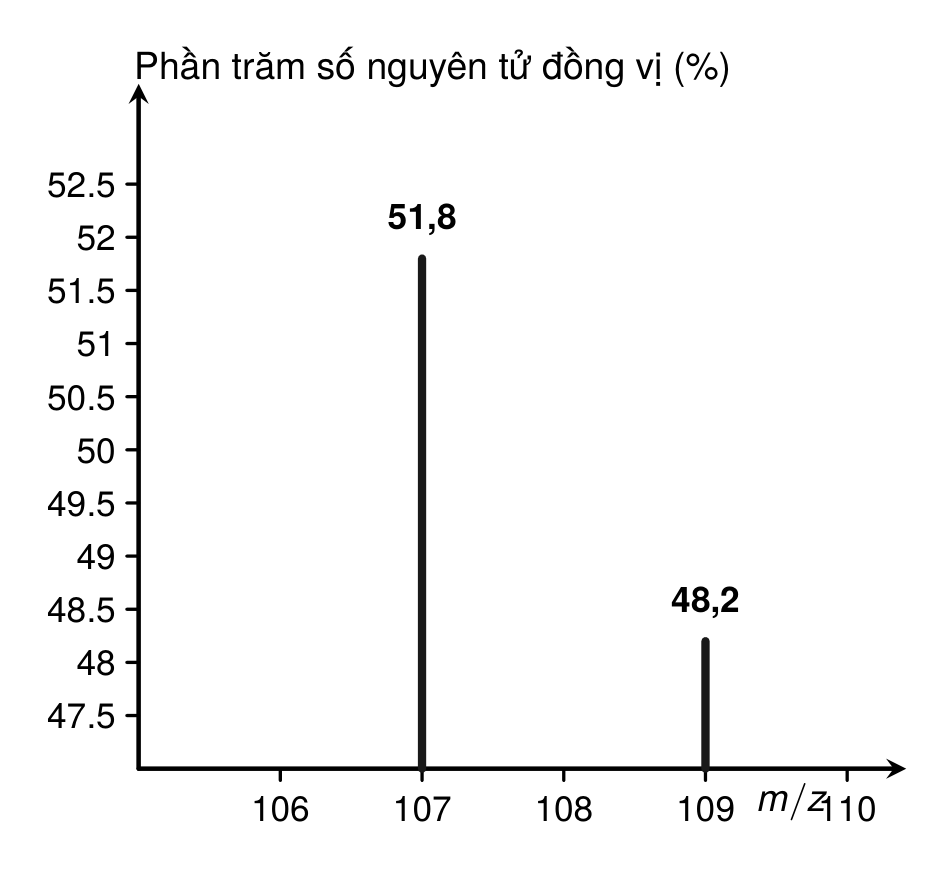
\includegraphics[width=6.5cm]{images_hoa10/pho_khoi_luong_silver_ag.png}
\end{center}
Nguyên tử khối trung bình của nguyên tố silver là
\choice
{108,012.}
{107,964.}
{108,000.}
{107,987.}
\end{ex}
\begin{ex}
Cho các phát biểu sau:\\
(a) Phân lớp 4s có mức năng lượng cao hơn phân lớp 3d.\\
(b) Trong mỗi orbital chỉ chứa tối đa 2 electron có chiều tự quay ngược nhau.\\
(c) Lớp M có 4 phân lớp.\\
(d) Số electron tối đa trong phân lớp 3d là 18.\\
(e) Số orbital của phân lớp s, p, d lần lượt là 1, 3, 5.\\
(f) Những electron ở gần hạt nhân có mức năng lượng cao nhất.\\
Số phát biểu đúng là
\choice
{5.}
{3.}
{2.}
{4.}
\end{ex}
\begin{ex}
Trong hạt nhân nguyên tử, hạt mang điện là
\choice
{proton và neutron.}
{proton.}
{electron.}
{proton và electron.}
\end{ex}
\begin{ex}
Dãy nào dưới đây gồm các đồng vị của cùng một nguyên tố hóa học?
\choice
{$^{40}_{18}\ce{X}, ^{40}_{19}\ce{Y}.$}
{$^{19}_{9}\ce{X}, ^{20}_{10}\ce{Y}.$}
{$^{14}_{6}\ce{X}, ^{14}_{7}\ce{Y}.$}
{$^{28}_{14}\ce{X}, ^{29}_{14}\ce{Y}.$}
\end{ex}
\begin{ex}
Nguyên tố hóa học là tập hợp các nguyên tử có cùng
\choice
{số hạt neutron.}
{tổng số hạt proton và neutron.}
{điện tích hạt nhân.}
{số khối.}
\end{ex}
\begin{ex}
Sự phân bố electron theo ô orbital nào dưới đây là đúng?
\choice
{$[\uparrow\uparrow]$}
{$[\uparrow\uparrow][\uparrow][\phantom{\uparrow}]$}
{$[\uparrow][\uparrow][\uparrow]$}
{$[\uparrow\downarrow][\uparrow][\phantom{\uparrow}]$}
\end{ex}
\begin{ex}
Cho cấu hình electron nguyên tử của một số nguyên tố như sau: $[\ce{Ne}]3s^2$, $[\ce{Ar}]3d^{10}4s^1$, $[\ce{Ar}]3d^{10}4s^2 4p^5$, $[\ce{He}]2s^2 2p^6$, $[\ce{Ar}]3d^7 4s^2$. Số nguyên tố thuộc nhóm A và nhóm B lần lượt là
\choice
{4; 1.}
{2; 2.}
{3; 2.}
{2; 3.}
\end{ex}
\begin{ex}
Nguyên tử X có 56 electron và 81 neutron. Kí hiệu nguyên tử của X là
\choice
{$^{137}_{56}\ce{X}$.}
{$^{56}_{81}\ce{X}$.}
{$^{81}_{56}\ce{X}$.}
{$^{112}_{56}\ce{X}$.}
\end{ex}
\begin{ex}
Số nguyên tố trong chu kì 3 và chu kì 5 lần lượt là
\choice
{18 và 18.}
{18 và 8.}
{8 và 18.}
{8 và 8.}
\end{ex}
\begin{ex}
Biết rằng một loại nguyên tử Sodium (Na) có 11 proton và 12 neutron. Phát biểu nào sau đây không đúng?
\choice
{Số khối của hạt nhân nguyên tử Sodium là 23.}
{Số hạt mang điện trong nguyên tử Sodium là 22.}
{Vỏ nguyên tử Sodium có 11 electron.}
{Điện tích hạt nhân nguyên tử Sodium là 11.}
\end{ex}
\begin{ex}
Nguyên tử của nguyên tố X có cấu hình electron là $\ce{1s^2 2s^1}$. Nguyên tố hóa học có cấu hình electron nào sau đây thuộc cùng một nhóm với nguyên tố X?
\choice
{$\ce{1s^2 2s^2 2p^1}$.}
{$\ce{1s^2 2s^2 2p^6 3s^2 3p^6 3d^5 4s^1}$.}
{$\ce{1s^2 2s^2 2p^6 3s^1}$.}
{$\ce{1s^2 2s^2 2p^6 3s^2 3p^1}$.}
\end{ex}
\begin{ex}
Nguyên tử của nguyên tố X có electron ở mức năng lượng cao nhất là 3p. Nguyên tử của nguyên tố Y có một electron ở lớp N. Nguyên tử X và Y có số electron hơn kém nhau là 3. Nguyên tử Y, X lần lượt là
\choice
{kim loại, phi kim.}
{kim loại, kim loại.}
{khí hiếm, kim loại.}
{phi kim, kim loại.}
\end{ex}
\begin{ex}
Nguyên tố X được sử dụng như một nguyên liệu cơ bản trong sản xuất phân bón. X là chất vô cùng cần thiết cho sự tăng trưởng và phát triển của các cây xanh. Ngoài những công dụng trên, X còn là một khoáng chất có vai trò rất quan trọng đối với sức khỏe con người. Nguyên tử của nguyên tố X có tổng số hạt (proton, electron, neutron) là 58, trong đó tổng số hạt mang điện nhiều hơn số hạt không mang điện là 18. Nguyên tử X có số hạt proton là
\choice
{19.}
{20.}
{38.}
{39.}
\end{ex}
\begin{ex}
Năm 1911, Rutherford cho chùm hạt $\alpha$ bắn vào một lá vàng rất mỏng và quan sát thấy hầu hết các hạt $\alpha$ đi thẳng qua lá vàng. Kết quả này chứng tỏ
\choice
{nguyên tử có cấu tạo rỗng.}
{hạt nhân nguyên tử mang điện tích âm.}
{electron có khối lượng rất lớn.}
{nguyên tử không chứa hạt mang điện.}
\end{ex}
\begin{ex}
Trong bảng tuần hoàn, chu kì gồm các nguyên tố mà nguyên tử của chúng có cùng
\choice
{số phân lớp electron.}
{cấu hình electron.}
{số electron hóa trị.}
{số lớp electron.}
\end{ex}
\vspace{4pt}
\noindent
{\color{mainGreen}\textbf{\large PHẦN II. Câu trắc nghiệm đúng sai}}\\
\textit{\small Học sinh trả lời từ câu 1 đến câu 2. Trong mỗi ý a), b), c), d) ở mỗi câu, học sinh chọn đúng hoặc sai.}
\vspace{2pt}

\begin{ex}
Sulfur dạng kem bôi được sử dụng để điều trị mụn trứng cá. Nguyên tử sulfur có phân lớp electron ngoài cùng là $\ce{3p^4}$.
\choiceTF
{Sulfur thuộc chu kì 3, nhóm VIA và là nguyên tố phi kim}
{Sulfur có số hiệu nguyên tử là 14}
{Nguyên tử $^{34}_{16}\ce{X}$ là đồng vị của sulfur}
{Ở trạng thái cơ bản, nguyên tử sulfur có 4 electron hóa trị}
\end{ex}
\begin{ex}
Hình dưới mô tả orbital (a) và orbital (b) chứa electron trong nguyên tử Sodium (Na) ở trạng thái cơ bản. Mức năng lượng của orbital (a) cao hơn orbital (b).
\begin{center}
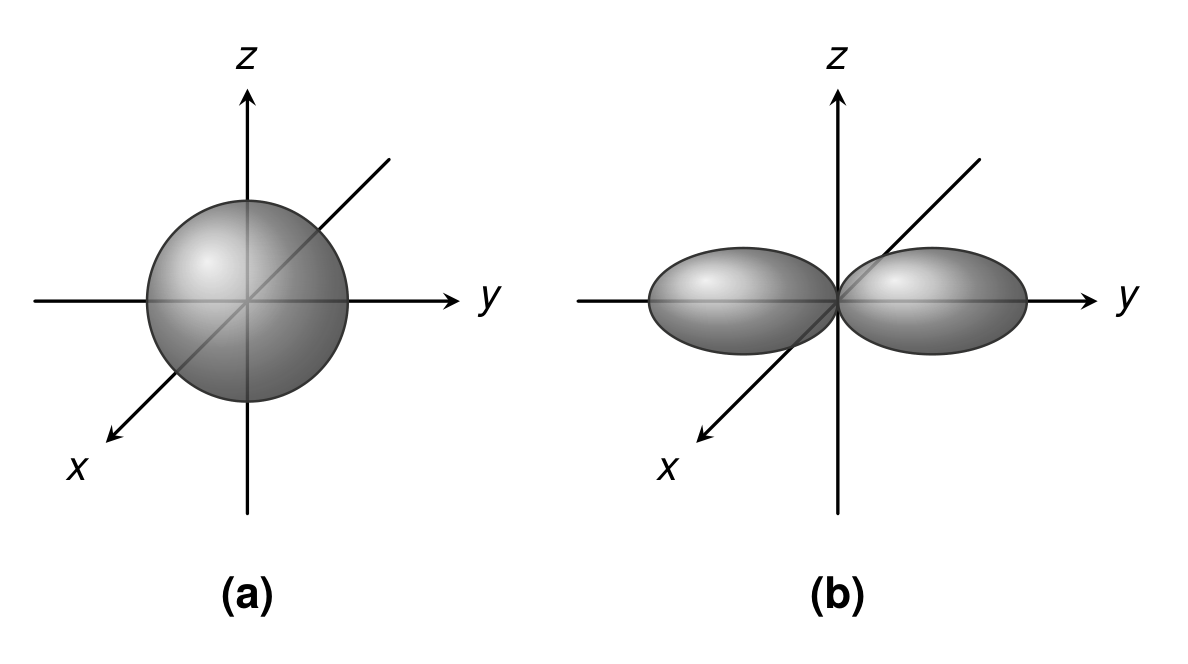
\includegraphics[width=8cm]{images_hoa10/hinh_orbital_s_va_p.png}
\end{center}
\choiceTF
{Số electron trong orbital (b) gấp đôi số electron trong orbital (a)}
{Số tám nổi (b) là hình dạng của AO p}
{Electron trên orbital (a) nằm gần hạt nhân hơn electron trên orbital (b)}
{Electron trong orbital (a) và (b) cùng thuộc 1 lớp electron}
\end{ex}
\vspace{4pt}
\noindent
{\color{mainGreen}\textbf{\large PHẦN III. Câu trắc nghiệm trả lời ngắn}}\\
\textit{\small Học sinh trả lời từ câu 1 đến câu 4.}
\vspace{2pt}

\begin{ex}
Khí carbon dioxide ($\ce{CO2}$) là nguyên nhân chính gây nên hiệu ứng nhà kính. Carbon có 2 đồng vị $^{12}_6\ce{C}, ^{13}_6\ce{C}$; oxygen có 3 đồng vị $^{16}_8\ce{O}, ^{17}_8\ce{O}, ^{18}_8\ce{O}$. Số loại phân tử $\ce{CO2}$ tạo thành là bao nhiêu?
\par\textbf{Trả lời:} \dotfill\end{ex}
\begin{ex}
Nguyên tố X thuộc chu kì 3, nhóm IIA. Nguyên tố Y thuộc cùng chu kì với X và thuộc nhóm VIIA. X và Y kết hợp với nhau tạo thành hợp chất có công thức $\ce{XY2}$. Tổng số proton có trong một phân tử $\ce{XY2}$ là bao nhiêu?
\par\textbf{Trả lời:} \dotfill\end{ex}
\begin{ex}
Cho các phát biểu sau:\\
(1) Nguyên tử có kích thước vô cùng nhỏ so với kích thước hạt nhân nguyên tử.\\
(2) Số khối của nguyên tử bằng tổng số proton và số neutron.\\
(3) Tất cả các nguyên tử đều chứa proton, electron và neutron.\\
(4) Khối lượng của nguyên tử tập trung hầu hết ở hạt nhân nguyên tử.\\
(5) Đồng vị là các nguyên tố có cùng số proton nhưng khác nhau số neutron.\\
Viết số thứ tự của các phát biểu đúng theo thứ tự tăng dần từ trái sang phải (ví dụ: 12 hoặc 123 hoặc 23...).
\par\textbf{Trả lời:} \dotfill\end{ex}
\begin{ex}
Cho 7 nguyên tố có số hiệu nguyên tử lần lượt là: 5, 18, 11, 13, 16, 19, 2. Trong các nguyên tố trên, có bao nhiêu nguyên tố là kim loại?
\par\textbf{Trả lời:} \dotfill\end{ex}
\vspace{6pt}
\noindent
{\color{mainGreen}\textbf{\Large B. PHẦN TỰ LUẬN (3 ĐIỂM)}}
\vspace{3pt}

\begin{ex}
Silicon (Si) được sử dụng trong nhiều ngành công nghiệp: gốm, men sứ, thủy tinh, luyện thép, vật liệu bán dẫn \dots\\
a) Viết cấu hình electron nguyên tử của nguyên tố silicon ($Z = 14$).\\
b) Xác định vị trí của silicon (ô nguyên tố, chu kì, nhóm) trong bảng tuần hoàn và giải thích.

\vspace{0.3cm}
\dotfill\\
\dotfill\\
\dotfill\\
\dotfill
\end{ex}
\begin{ex}
Cho X, Y, T là ba nguyên tố liên tiếp nhau trong một chu kì của bảng tuần hoàn các nguyên tố hóa học. Tổng số các hạt mang điện trong thành phần cấu tạo nguyên tử của X, Y, T bằng 72. Xác định số hiệu nguyên tử của các nguyên tố X, Y, T?

\vspace{0.3cm}
\dotfill\\
\dotfill\\
\dotfill\\
\dotfill\\
\dotfill
\end{ex}
\begin{ex}
Một nguyên tố R có 3 đồng vị X, Y, Z, tổng số hạt electron, proton và neutron của 3 đồng vị bằng 111. Số neutron của đồng vị X bằng số proton, số neutron của đồng vị Z hơn đồng vị Y 1 hạt.\\
a) Xác định số khối của 3 đồng vị.\\
b) Cho biết tỷ lệ số nguyên tử của các đồng vị như sau: $\ce{X : Y} = 393 : 50$ và $\ce{Y : Z} = 50 : 57$, xác định nguyên tử khối trung bình của R và khối lượng của $9,033 \cdot 10^{22}$ nguyên tử R.\\
\textit{(Biết số Avogadro $= 6,022 \cdot 10^{23}$)}

\vspace{0.3cm}
\dotfill\\
\dotfill\\
\dotfill\\
\dotfill\\
\dotfill\\
\dotfill
\end{ex}
\vspace{6pt}
\begin{center}
\textbf{---------- HẾT ----------}\\
\textit{\small - Học sinh không được sử dụng tài liệu.\\
- Cán bộ coi thi không giải thích gì thêm.}
\end{center}
\end{document}
